\documentclass[10pt,a4paper]{article}
\usepackage[utf8x]{inputenc}
\usepackage[ngerman]{babel}
\usepackage{amsmath}
\usepackage{amsfonts}
\usepackage{amssymb}
\usepackage{pdfpages}
\usepackage{multirow}
\usepackage[linkbordercolor=white,linkcolor=black ]{hyperref}
\usepackage{lscape}

\begin{document}

\newcommand{\abs}[1]{\ensuremath{\left\vert#1\right\vert}}

\newcommand{\ENDV}{\hspace{5mm} \vline \hspace{1mm}}
\newcommand{\LHospital}{\stackrel{L'H}{=}}
\newcommand{\two}{\nodepart{two}}
\newcommand{\three}{\nodepart{three}}
\newcommand{\four}{\nodepart{four}}
\newcommand{\TablePos}{!htbp}
\newcommand{\LargeRowSize}{\renewcommand{\arraystretch}{1.5}}
\newcommand{\largeRowSize}{\renewcommand{\arraystretch}{1.2}}
\newcommand{\normalRowSize}{\renewcommand{\arraystretch}{1}}
\newcommand{\DefaultTabular}{|c|c|p{9cm}|}

\title{Statistik Zusammenfassung}
\author{Nils Weiß - Alexander Strobl}

\maketitle
\tableofcontents

\newpage
\section{Grundlagen}

\subsection{Häufigkeitsverteilungen}

\begin{figure}[!h]
\begin{tabular}{|c|p{8cm}|} 
\hline Eigenschaft & Beschreibung \\ 
\hline Merkmalsträger & Objekt von Interesse bei empirischer Untersuchung\\ 
\hline Gesamtheit & Menge der relevanten Merkmalsträger. Die Anzahl nennt man Umfang der Gesamtheit \\
\hline Mikrodaten & Daten, welche ausgewertet werden sollen \\
\hline Häufigkeitsverteilung & Ausprägungen der einzelnen Merkmalsträger \\
\hline
\end{tabular}
\caption{Begriffserklärungen: Häufigkeitsverteilung}
\end{figure}

\begin{figure}[!h]
\begin{tabular}{|p{3cm}|p{3cm}|p{3cm}|} 
\hline Merkmalsausprägung $x_i$ & absolute Häufigkeiten $n_i$ & relative Häufigkeiten $f_i$ \\
\hline 1 & 6 & 0.3 / 30\% \\
\hline 2 & 7 & 0.35 / 35\% \\
\hline 3 & 4 & 0.2 / 20\%\\
\hline 4 & 2 & 0.1 / 10 \%\\
\hline 5 & 1 & 0.05 / 5 \%\\
\hline $\sum$ & 20 & 1 / 100 \%\\
\hline 
\end{tabular}
\caption{Beispiel: Häufigkeitsverteilung von Noten}
\end{figure}

\subsection{Kummulierte Häufigkeiten}
\subsubsection{Absolut}

Summe der ``ersten" $i$ absoluten Häufigkeiten\\

$N_i = \sum\limits^i_{j = 1}n_j$

\subsubsection{Relativ}

Summe der ``ersten" $i$ relativen Häufigkeiten\\

$F_i = \sum\limits^i_{j=1}f_j$

\subsubsection{Empirische Verteilungsfunktion}

Summe über alle $i$, für die $x_i \leqslant x$ ist \\
Es werden die relativen Häufigkeiten $f_i$ all jener Ausprägungen summiert, die 
höchsten gleich $x$ sind\\

$F(x) = \sum\limits_{\{i|x_i \leqslant x\}} f_i$

\begin{figure}[!h]
\begin{tabular}{|p{2cm}|p{2cm}|p{2cm}|p{3cm}|p{4cm}|} 
\hline Klasse i $x_i$ & Klassen-obergrenze $x_i^o$ & abs. Häufigkeiten $n_i$ & rel. Häufigkeiten $f_i$ & emp. Verteilungsfunktion a. d. Klassenobergrenze $F(x_i^0)$ \\
\hline 1 & 29 & 7 & 0.01165 & 1.17 \% \\
\hline 2 & 39 & 59 & 0.09817 & 10.98 \%  \\
\hline 3 & 49 & 127 & 0.21131 & 32.11 \%\\
\hline 4 & 54 & 120 & 0.19967 & 52.08 \%\\
\hline 5 & 59 & 146 & 0.24293 & 76.37 \%\\
\hline 6 & 64 & 112 & 0.18636 & 95.01 \%\\
\hline 7 & 73 & 30 & 0.04992 & 100.00 \%\\
\hline $\sum$ & & 601 & 1 & \\
\hline 
\end{tabular}
\caption{klassierte Altersverteilung}
\end{figure}

\subsection{Maßzahlen zur Beschreibung einer Verteilung}
\subsubsection{Modus}
(auch: Modalwert, häufigster Wert)

Bezeichnet das Merkmal $x_i$ mit der größten absoluten Häufigkeit $n_i$ bzw. der 
größten relativen Häufigkeit $f_i$.

\subsubsection{Median - Quantile}

Median: $x_{0,5}$= 50\% Quantil\\

Wichtige Quantile: $x_{0,25}$, $x_{0,75}$

\subsubsection{Arithmetisches Mittel}
(auch: Mittelwert, Durchschnittswert)\\

$\overline{x} = \frac{\textbf{Summe aller Merkmalswerte}}{\textbf{Anzahl aller 
Merkmalswerte}}$\\

$\overline{x} = \frac{1}{n} \sum\limits_{i=1}^{n} x_i$\\

$\overline{x} = \frac{1}{n} \sum\limits_{i=1}^{k} x_i n_i$\\

$\overline{x} = \sum\limits_{i=1}^{k} x_i f_i$\\

$\overline{x} = \frac{1}{n} \sum\limits_{i=1}^{r} \overline{x_i} n_i$\\

$\overline{x} = \sum\limits_{i=1}^r \overline{x_i} f_i$\\
\newpage
\section{Streuung und Konzentration}

\subsubsection{Spannweite}
(Einfachstes Streuungsmaß, Differenz zwischen größtem und kleinstem auftretenden 
Merkmalswert)\\

$\textbf{Spannweite} = max(x_i) - min(x_i)$

\subsubsection{Quartilsabstand}
(Spannweite der mittleren 50\% der Merkmalsträger)\\

$\textbf{Quartilsabstand} = x_{0,75} - x_{0,25}$

\subsubsection{Varianz}
(Mittlere quadratische Abweichung vom Mittelwert)\\

$s^2 = \frac{1}{n}\sum\limits_{i=1}^n (x_i - \overline{x})^2 = \frac{1}{n}\sum\limits_{i=1}^k (x_i - \overline{x})^2 n_i = \sum\limits_{i=1}^k (x_i - \overline{x})^2 f_i$ \\

$s^2 = \frac{1}{n}\sum\limits_{i=1}^n x_i^2 - \overline{x}^2 = \frac{1}{n}\sum\limits_{i=1}^k x_i^2 n_i - \overline{x}^2 = \sum\limits_{i=1}^k x_i^2 f_i - \overline{x}^2$ \\

$s^2 = \overline{x^2} - \overline{x}^2$\\

\textbf{Varianz bei Vorliegen von Teilgesamtheiten}\\

$s^2 = \frac{1}{n}\sum\limits_{i=1}^r s_i^2n_i +  \frac{1}{n}\sum\limits_{i=1}^r (\overline{x_i} - \overline{x})^2 n_i $

\subsubsection{Standardabweichung}

$s = \sqrt{s^2}$

\subsubsection{Standardisierte Merkmale}

Ein Merkmal, für dessen Verteilung $\overline{x} = 0$ und $s^2 = 1$ gilt, heißt 
standardisiert.

\subsubsection{Kovarianz}
(von X und Y)\\

$s_{XY} = \frac{1}{n} \sum\limits_{i=1}^n (x_i - \overline{x})(y_i - \overline{y}) 
= \frac{1}{n} \sum\limits_{i=1}^n x_i y_i - \overline{x} ~ \overline{y}$

\subsubsection{Korrelationskoeffizient}
(nach Bravais-Pearson)\\

$\frac{s_{XY}}{s_X s_Y} = 
 \frac{  \frac{1}{n} \sum\limits_{i=1}^n (x_i - \overline{x})(y_i - \overline{y}) }
 {\sqrt{\frac{1}{n} \sum\limits_{i=1}^n (x_i - \overline{x})^2} \sqrt{\frac{1}{n} \sum\limits_{i=1}^n (y_i - 
 \overline{y})^2}}$\\
 
 Es gilt: $-1 \leqslant r \leqslant 1$
 
 $r = 0$: kein linearer Zusammenhang
 $r = 1$: steigende Gerade
 $r = -1$: fallende Gerade 
 
 \subsubsection{Regressionsgerade}
 
 $\hat{y} = \hat{\alpha} + \hat{\beta}x$\\
 
 $\hat{\beta} = \frac{s_{XY}}{s_X}$\\
 
 $\hat{\alpha} = \overline{y} - \hat{\beta}\overline{x}$\\
 
\section{Wahrscheinlichkeitstheorie}
\LargeRowSize
\begin{table}[!h]
\begin{tabular}{\DefaultTabular}
\hline \textbf{Eigenschaft} & \textbf{Formel} \\
\hline Wahrscheinlichkeitsraum & $\Omega$ \\
\hline LaPlace-Wahrscheinlichkeit & $P(A) = \frac{\text{Anz. Elem in A}}{\text{Anz. Elem in }\Omega} = \frac{\abs A}{\abs \Omega}$ \\
\hline Bedingte Wahrscheinlichkeiten & $P(B | A) = \frac{P(A \cap B)}{P(A)}$ \\
\hline Multiplikationssatz & $P(A \cap B) = P(A) * P(B|A)$ \\
\hline Additionssatz (bel. Ereignisse) & $P(A \cup B) = P(A) + P(B) - P(A \cap B)$ \\
\hline Additionssatz (ausschließende Ereignisse) & $P(A \cup B) = P(A) + P(B)$ // \textbf{( A $\cap$ B = $\emptyset$)} \\
\hline Abhängigkeit & $P(A\cup B) = P(A) + P(B) - P(A)P(B)$  \\
\hline Unabhängigkeit & $P(A\cap B) = P(A)P(B)$  \\
\hline Totale Wahrscheinlichkeit & $P(B) = \sum\limits_{i=1}^mP(B\cap A_) = P(A_i)P(B|A_i)$  \\
\hline Satz von Bayes & $P(A_j|B) = \frac{P(B|A_j)P(A_j)}
{\sum\limits_{i=1}^m P(B|A_i)P(A_i)}$  \\
\hline
\end{tabular}
\caption{Begriffserklärungen: Wahrscheinlichkeitstheorie}
\end{table}
\normalRowSize
\newpage

\begin{landscape}
\section{Diskrete Zufallsvariablen}
\LargeRowSize
\begin{table}[!h]
\begin{tabular}{\DefaultTabular}
\hline Eigenschaft & Formel & Beschreibung \\
\hline Verteilungsfunktion & $F_x(x) = P(X \leq x)$ & definiert die Wahrscheinlichkeit der Zufallsvariable X, dass X höchstens den Wert x annimmt\\
\hline \multirow{2}{*}{Unabhängigkeit} & $P(X_1 = x_1, X_2 = x_2)$ & \multirow{2}{*}{gilt ebenfalls für andere Operationen wie z.B. $\leq$} \\
 & $= P(X_1 = x_1) * P(X_2 = x_2)$ & \\
\hline \multirow{2}{*}{Erwartungswert} & E(X) = $\mu_x$ = $\mu$ & \multirow{2}{*}{Ist der Mittelwert von X} \\
& $= \sum\limits_{i=1}^k x_i p_i = \sum\limits_{i=1}^k x_i* P(X = x_i)$ & \\
& & Weitere Rechenregeln:\\
& E(Y) = E(g(X)) = $\sum\limits_i g(x_i)p_i$ & Wenn g(x) eine reelle Funktion und Y = g(X) \\
& E(X + Y) = E(X) + E(Y) & \\
& $E\left(\sum\limits_{i=1}^n X_i\right) = \sum\limits_{i=1}^nE(X_i)$ & \\ 
\hline Varianz & $Var(X) = E((X - \mu_x)^2)$ & \\
\cline{2-3} & $= \sum\limits_{i=1}^k(x_i - \mu_x)^2*p_i$ & \\
\cline{2-3} & $=E(X^2) - E(X)^2$ &\\
\hline
\end{tabular}
\caption{Begriffserklärungen: Diskrete Zufallsvariablen}
\end{table}
\end{landscape}
\normalRowSize
\newpage

\begin{landscape}
\section{Stetige Zufallsvariablen}
\LargeRowSize
\begin{table}[!h]
\begin{tabular}{\DefaultTabular}
\hline Eigenschaft & Formel & Beschreibung \\
\hline \multirow{4}{*}{Definition} & $F_x(x) = \int\limits_{-\infty}^{x}f(t)dt$ & Verteilungsfunktion, $f(t) =$ Dichtefunktion\\
\cline{2-3} &  $P(X = x) = 0$ & Wahrscheinlichkeit für einen Wert gleich x ist immer 0\\
\cline{2-3} & $P(x_1 \leq X \leq x_2) = F_x(x_2) - F_x(x_1)$ & $F_x^{'}(x) = f_x(x)$ Die Dichtefunktion ist die Ableitung der Verteilungsfunktion \\
\hline Erwartungswert $\mu_x$ & $E(X) = \int\limits_{-\infty}^{+\infty} x*f(x)dx$ & Die Dichtefunktion $f(x)$ wird nie verändert! \newline $E(\frac{1}{X}) = \int \frac{1}{X}*f(x)dx$\\
\hline \multirow{3}{*}{Rechenregeln} & $E(Y) = E(g(X)) = \int\limits_a^bg(x)*f(x)dx$ & $g(x)$ ist eine reelle Funktion\\
\cline{2-3} & $E(aX + b) = a*E(X) + b$ & lineare Transformation\\
\cline{2-3} & $E(X+Y) = E(X) + E(Y)$ & \\
\hline Modus & $F_x(x_p) = p$ & Die Wahrscheinlickeit, dass X höchstens den Wert $x_p$ annimmt, ist mind. $p/100 \%$ \\
\hline Varianz & $Var(X) = \int\limits_{-\infty}^{+\infty}(x-\mu_x)^2*f(x)dx$ & Standardabweichung ist $\sqrt{Var(X)}$\\
\hline Rechenregeln & vgl. Diskrete Zufallsvariablen & \\
\hline
\end{tabular}
\caption{Begriffserklärungen: Stetige Zufallsvariablen}
\end{table}
\end{landscape}

\normalRowSize

\newpage
\begin{landscape}
\section{Diskrete Verteilungen}
\begin{figure}[H]
\centering
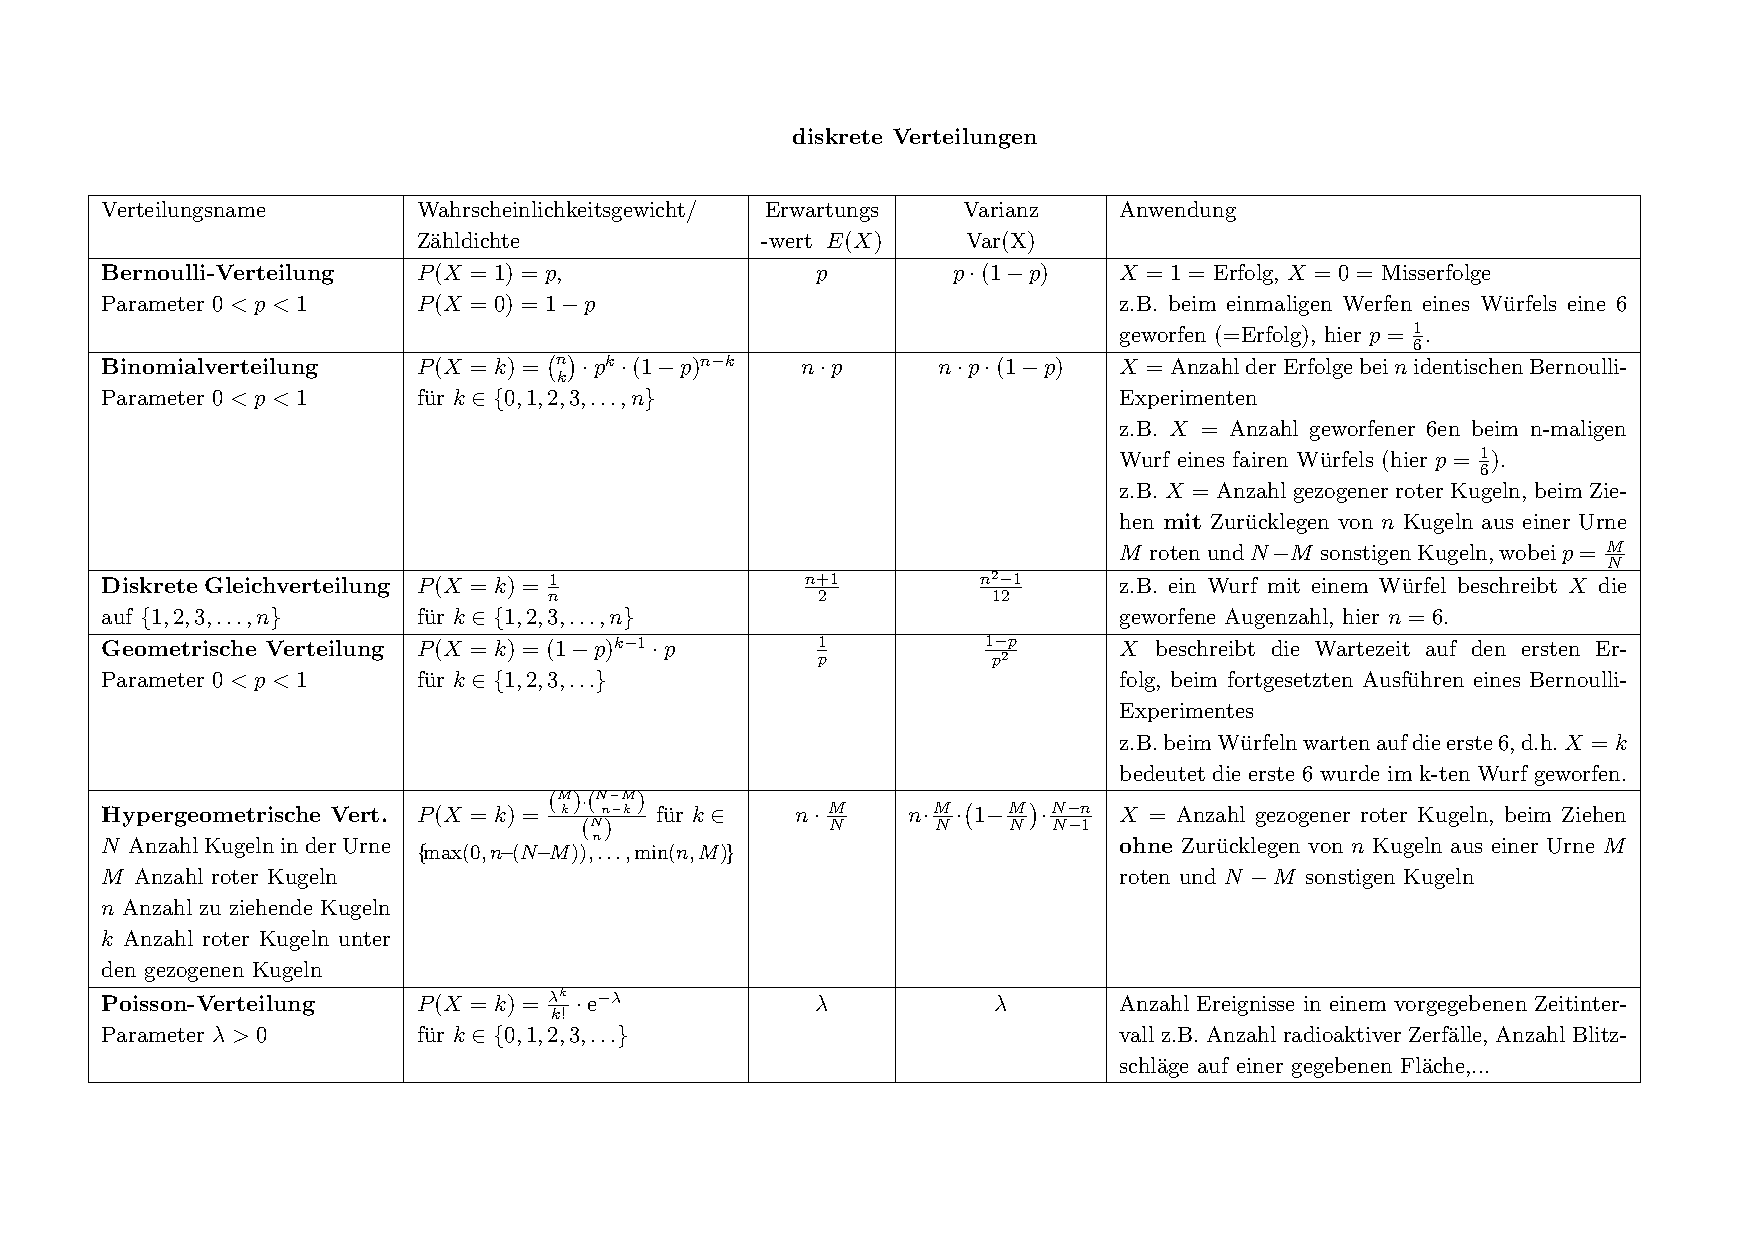
\includepdf[page=1, angle=90, scale = 0.7]{Zusammenfassung_Verteilungen}
\end{figure}
\end{landscape}

\begin{landscape}
\section{Stetige Verteilungen}
\begin{figure}[H]
\centering
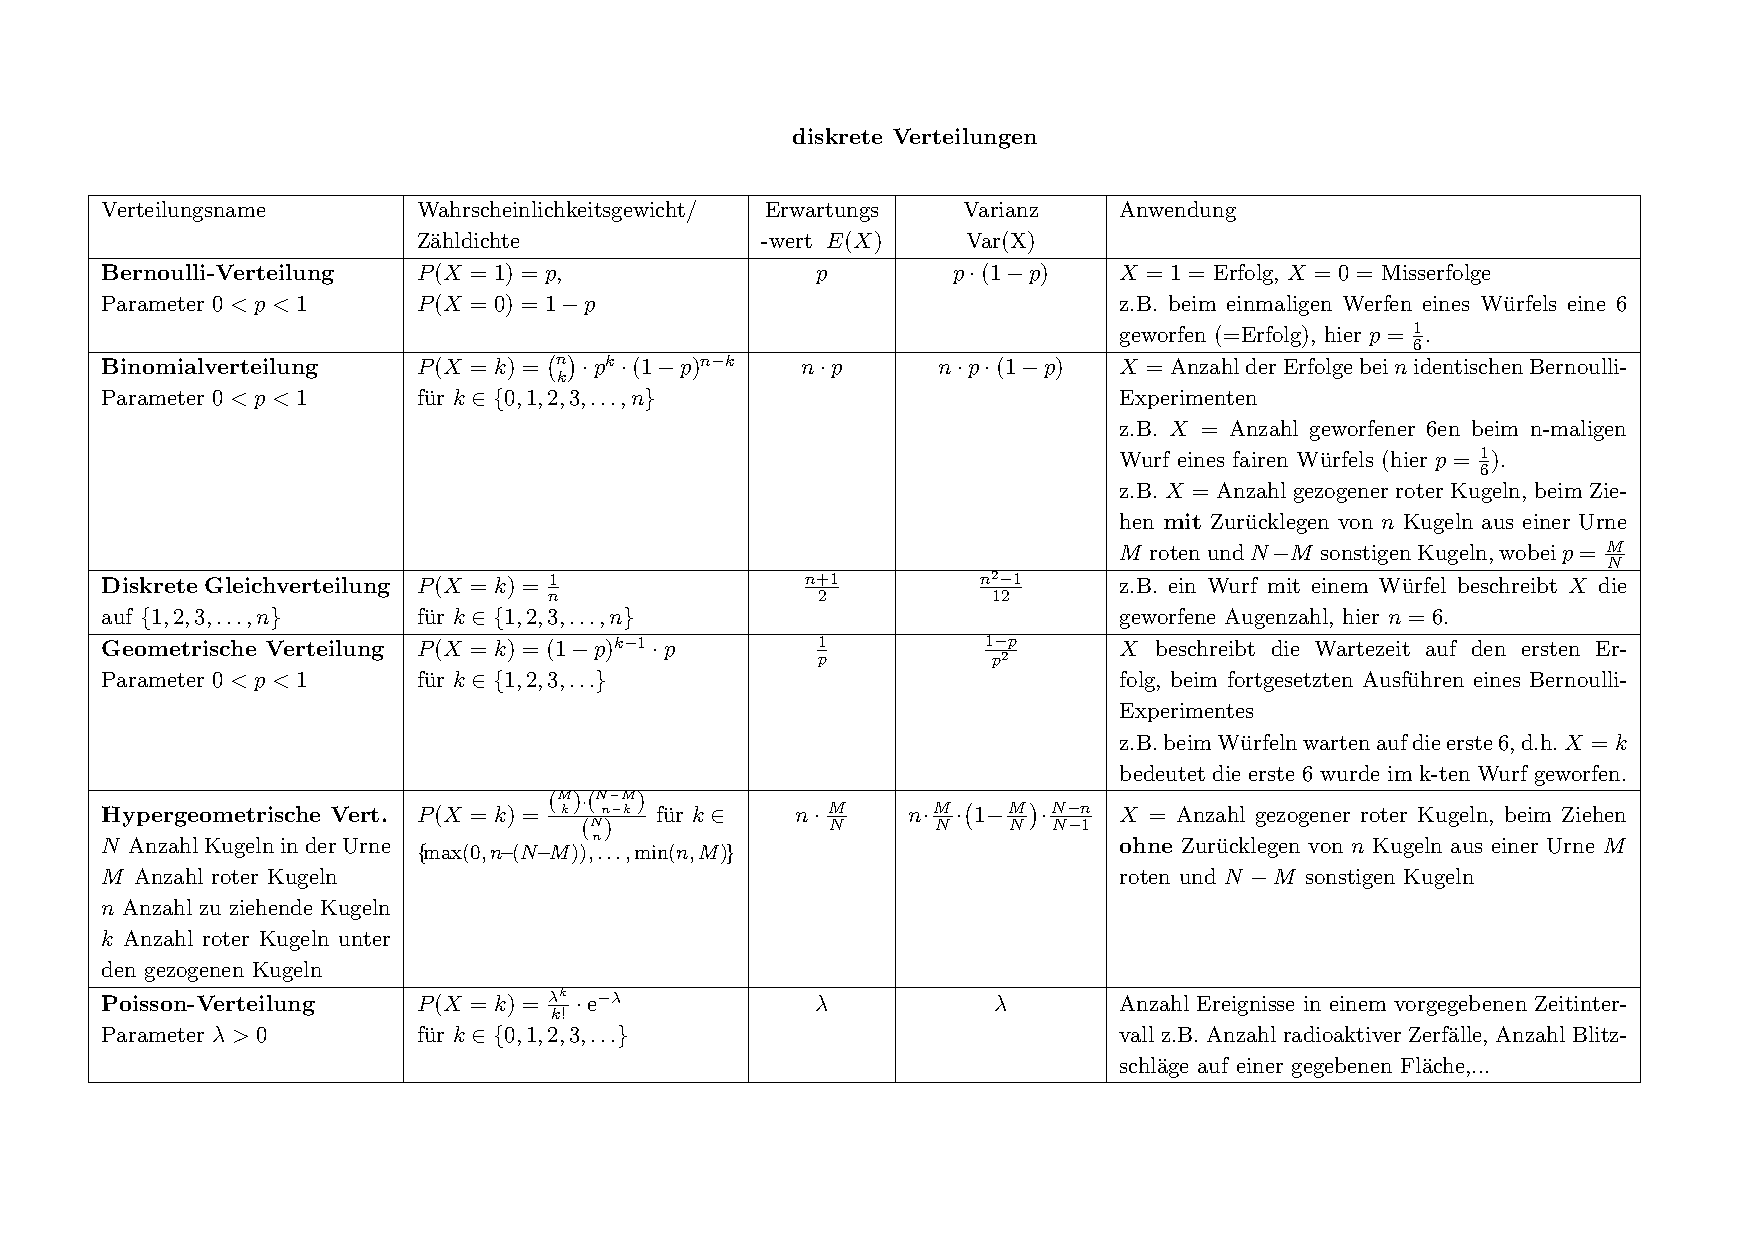
\includepdf[page=2, angle=90, scale = 0.7]{Zusammenfassung_Verteilungen}
\end{figure}
\end{landscape}

\end{document}




